\documentclass[conference]{IEEEtran}
\IEEEoverridecommandlockouts
% The preceding line is only needed to identify funding in the first footnote.
%If that is unneeded, please comment it out. Template version as of 6/27/2024

\usepackage{cite}
\usepackage{amsmath,amssymb,amsfonts}
\usepackage{algorithmic}
\usepackage{graphicx}
\usepackage{textcomp}
\usepackage{xcolor}
\bibliographystyle{IEEEtran}
\def\BibTeX{{\rm B\kern-.05em{\sc i\kern-.025em b}\kern-.08em
    T\kern-.1667em\lower.7ex\hbox{E}\kern-.125emX}}
\begin{document}

\title{Forecasting microclimates with a low-cost LoRa enabled weather station
network\\
\thanks{Identify applicable funding agency here. If none, delete this.}
}

\author{\IEEEauthorblockN{1\textsuperscript{st} Adam Sidnell}
\IEEEauthorblockA{\textit{Computer Science MSc} \\
\textit{University of Bristol}\\
Bristol, United Kingdom \\
adam.sidnell@gmail.com}
\and
\IEEEauthorblockN{2\textsuperscript{nd} Ruzanna Chitchyan}
\IEEEauthorblockA{\textit{Professor in Computer Science} \\
\textit{University of Bristol}\\
Bristol, United Kingdom \\
r.chitchyan@bristol.ac.uk} }

\maketitle

\begin{abstract}
Farmers require accurate weather forecasting for a variety of reasons. Such as
deciding if wind speed will be low enough to spray crops or whether there is a
risk of spring frost and they should take appropriate action. This paper
develops a low-cost weather station network built from widely available
electronics for deployment in an agricultural setting. It then uses data from
the network to train a LightGBM 
\end{abstract}

\begin{IEEEkeywords}
machine learning, smart farming, forecast, microclimate, IoT, LoRa, LightGBM
\end{IEEEkeywords}

\section{Introduction}\label{INTRO} 

\section{Related Work}\label{REL}

\subsection{LoRa based IoT in agriculture}

IoT devices have seen widespread adoption in agriculture, with digital solutions
offering the potential to improve yields even in remote areas. LoRa is an
especially relevant technology in this context as the range of these devices
enables data to be transmitted over long distances; additionally the low power
of these devices allows for the use of gridless power solutions - such as
solar-battery as used here. 

There are relatively few papers examining the effectiveness of LoRa in
agriculture but some notable examples include \cite{edgeAiGiaEtAl} where LoRa
was used in an edge computing exercise. In this study the authors used CNN
machine learning to create a compressed image that holds thousands of simulated
climate readings. This image can then be sent over LoRa to a receiver node which
can infer the readings of each node from this single image. While only one
sensor node was created for the exercise they also tested the range of this
device at a distance of 200m. This system would be useful in particularly large
networks of LoRa devices where the low data transfer speed of LoRa would start
to be a limiting factor.

The authors in \cite{smartFarmKodaliEtAl} implement a LoRa based weather station
prototype in India. The authors create a node that measures temperature,
humidity and soil moisture in an experimental setting with no field deployment.
Readings are then sent via LoRa to a receiver and can be read manually from the
device's screen or viewed on an IBM dashboard.  

\subsection{Weather forecasting microclimates with machine learning}

General weather models operate at magnitudes between 1 and 10 km and
microclimate predictions require models that operate at scales of roughly 100m
or less. Using existing general forecast models for micro-scale predictions is
computationally expensive \cite{blunn2024machine}, and these models have lower
accuracy rates than predictions using machine learning due to the inherent
complexity and non-linear nature of microclimates. Therefore a number of studies
have focused on building bespoke models to predict very local forecasts using
machine learning processes.

A 2021 study by Kumar et al \cite{kumar2021} developed an ML framework called
DeepMC as a part of a Microsoft Research initiative. Their model is able to
predict a variety of climatic variables such as soil moisture, wind speed and
temperature using inputs from weather station forecasts and IoT sensors. They
were able to get up to 90\% accuracy with a 12-120 hour forecast range.

Zanchi et al \cite{zanchi2023harnessing} used physical modelling of local
terrain combined with deep learning (DL) to forecast the microclimate in the
foothills of Lombardy. The objective was to predict the local conditions at the
meter-scale as opposed to the 10km+ scale of regional and global weather
forecasts. The initial model combined data about the morphology of the local
terrain and weather forecast data to provide the input data for two feed-forward
neural networks. These neural networks were trained to predict the local weather
variables using data from 25 sensors deployed in the region being studied.  The
study demonstrated that local predictions were more accurate when using forecast
data from local weather stations as opposed to global climate datasets, but
accuracy good in both.

Blunn et al \cite{blunn2024machine} ran a study focussed on predicting
temperatures in urban environments during heatwaves, using data from eight
heatwaves in London, UK. They used data from the UKV - a high-resolution weather
forecasting model - and from citizen weather stations (CWS). The authors used a
similar model training design to that in this study. A number of ML models were
trained on UKV variables (i.e. a general forecast) and CWS variables (local
sensor data) to bias correct the UKV readings and create a forecast prediction
model that could predict the CWS readings accurately (mean average error:
0.12\(^\circ\)C) compared with the general weather readings from UKV (mean
average error: 0.64\(^\circ\)C). The main points of difference to this paper are
the use of only temperature versus a wider range of variables in this study,
along with the use of custom weather stations here compared to public weather
data.

A recent paper from Abdelmadjid et al 2025 \cite{abdelmadjid2025enhancing} used
online datasets from Kaggle (a public repository of various datasets) to develop
an ML tool to predict changes in temperature and humidity within greenhouses in
response to changes to external weather conditions.  They used this data to test
three ML models and three DL models and selected the LightGBM ML model and the
LSTM DL model as the best performing models for prediction. The overall system
design consisted of four LSTM models feeding into the LightGBM model. This
design resulted in 98.45\% accuracy for temperature predictions and 99.61\%
accuracy for humidity predictions. Due to these results LightGBM was also chosen
for this experiment.

\section{Methodology}\label{METH}

\subsection{IoT hardware}

\begin{figure}[htbp]
\centerline{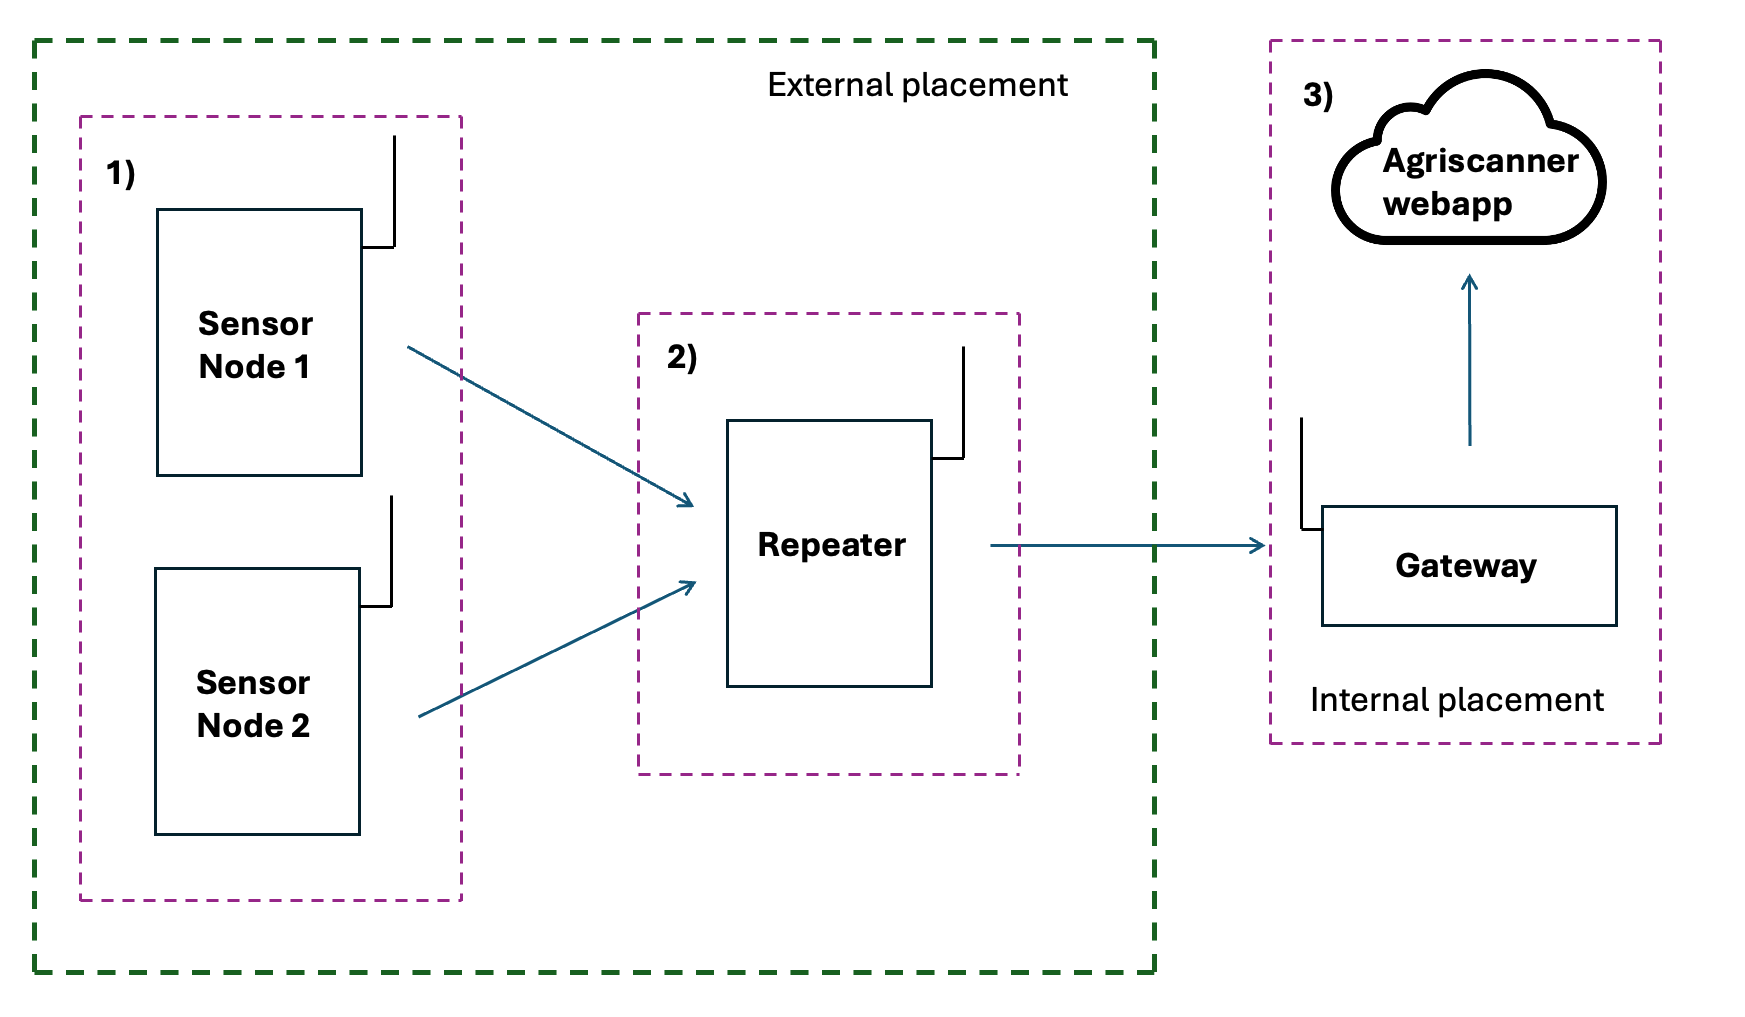
\includegraphics[width=0.5\textwidth]{figures/network-diagram.png}}
\caption{Network diagram of the system}
\label{fig}
\end{figure}

The design of the hardware consisted of two sensor nodes, a repeater and a
gateway. The purpose for each is outlined below:

\begin{enumerate}
    \item Sensor node: Collects temperature, humidity, wind speed and soil
    moisture data every 6 seconds. These readings are then averaged and sent as
    a single packet each minute to the repeater. Figure \ref{sensor-node}
    \item Repeater: Receives LoRa signals from the sensor nodes and then
    immediately re-transmits these to boost range. 
    \item Gateway: A hub that receives LoRa signals and then transmits weather
    data using WIFI.
\end{enumerate}

\begin{figure}[htbp]
\centerline{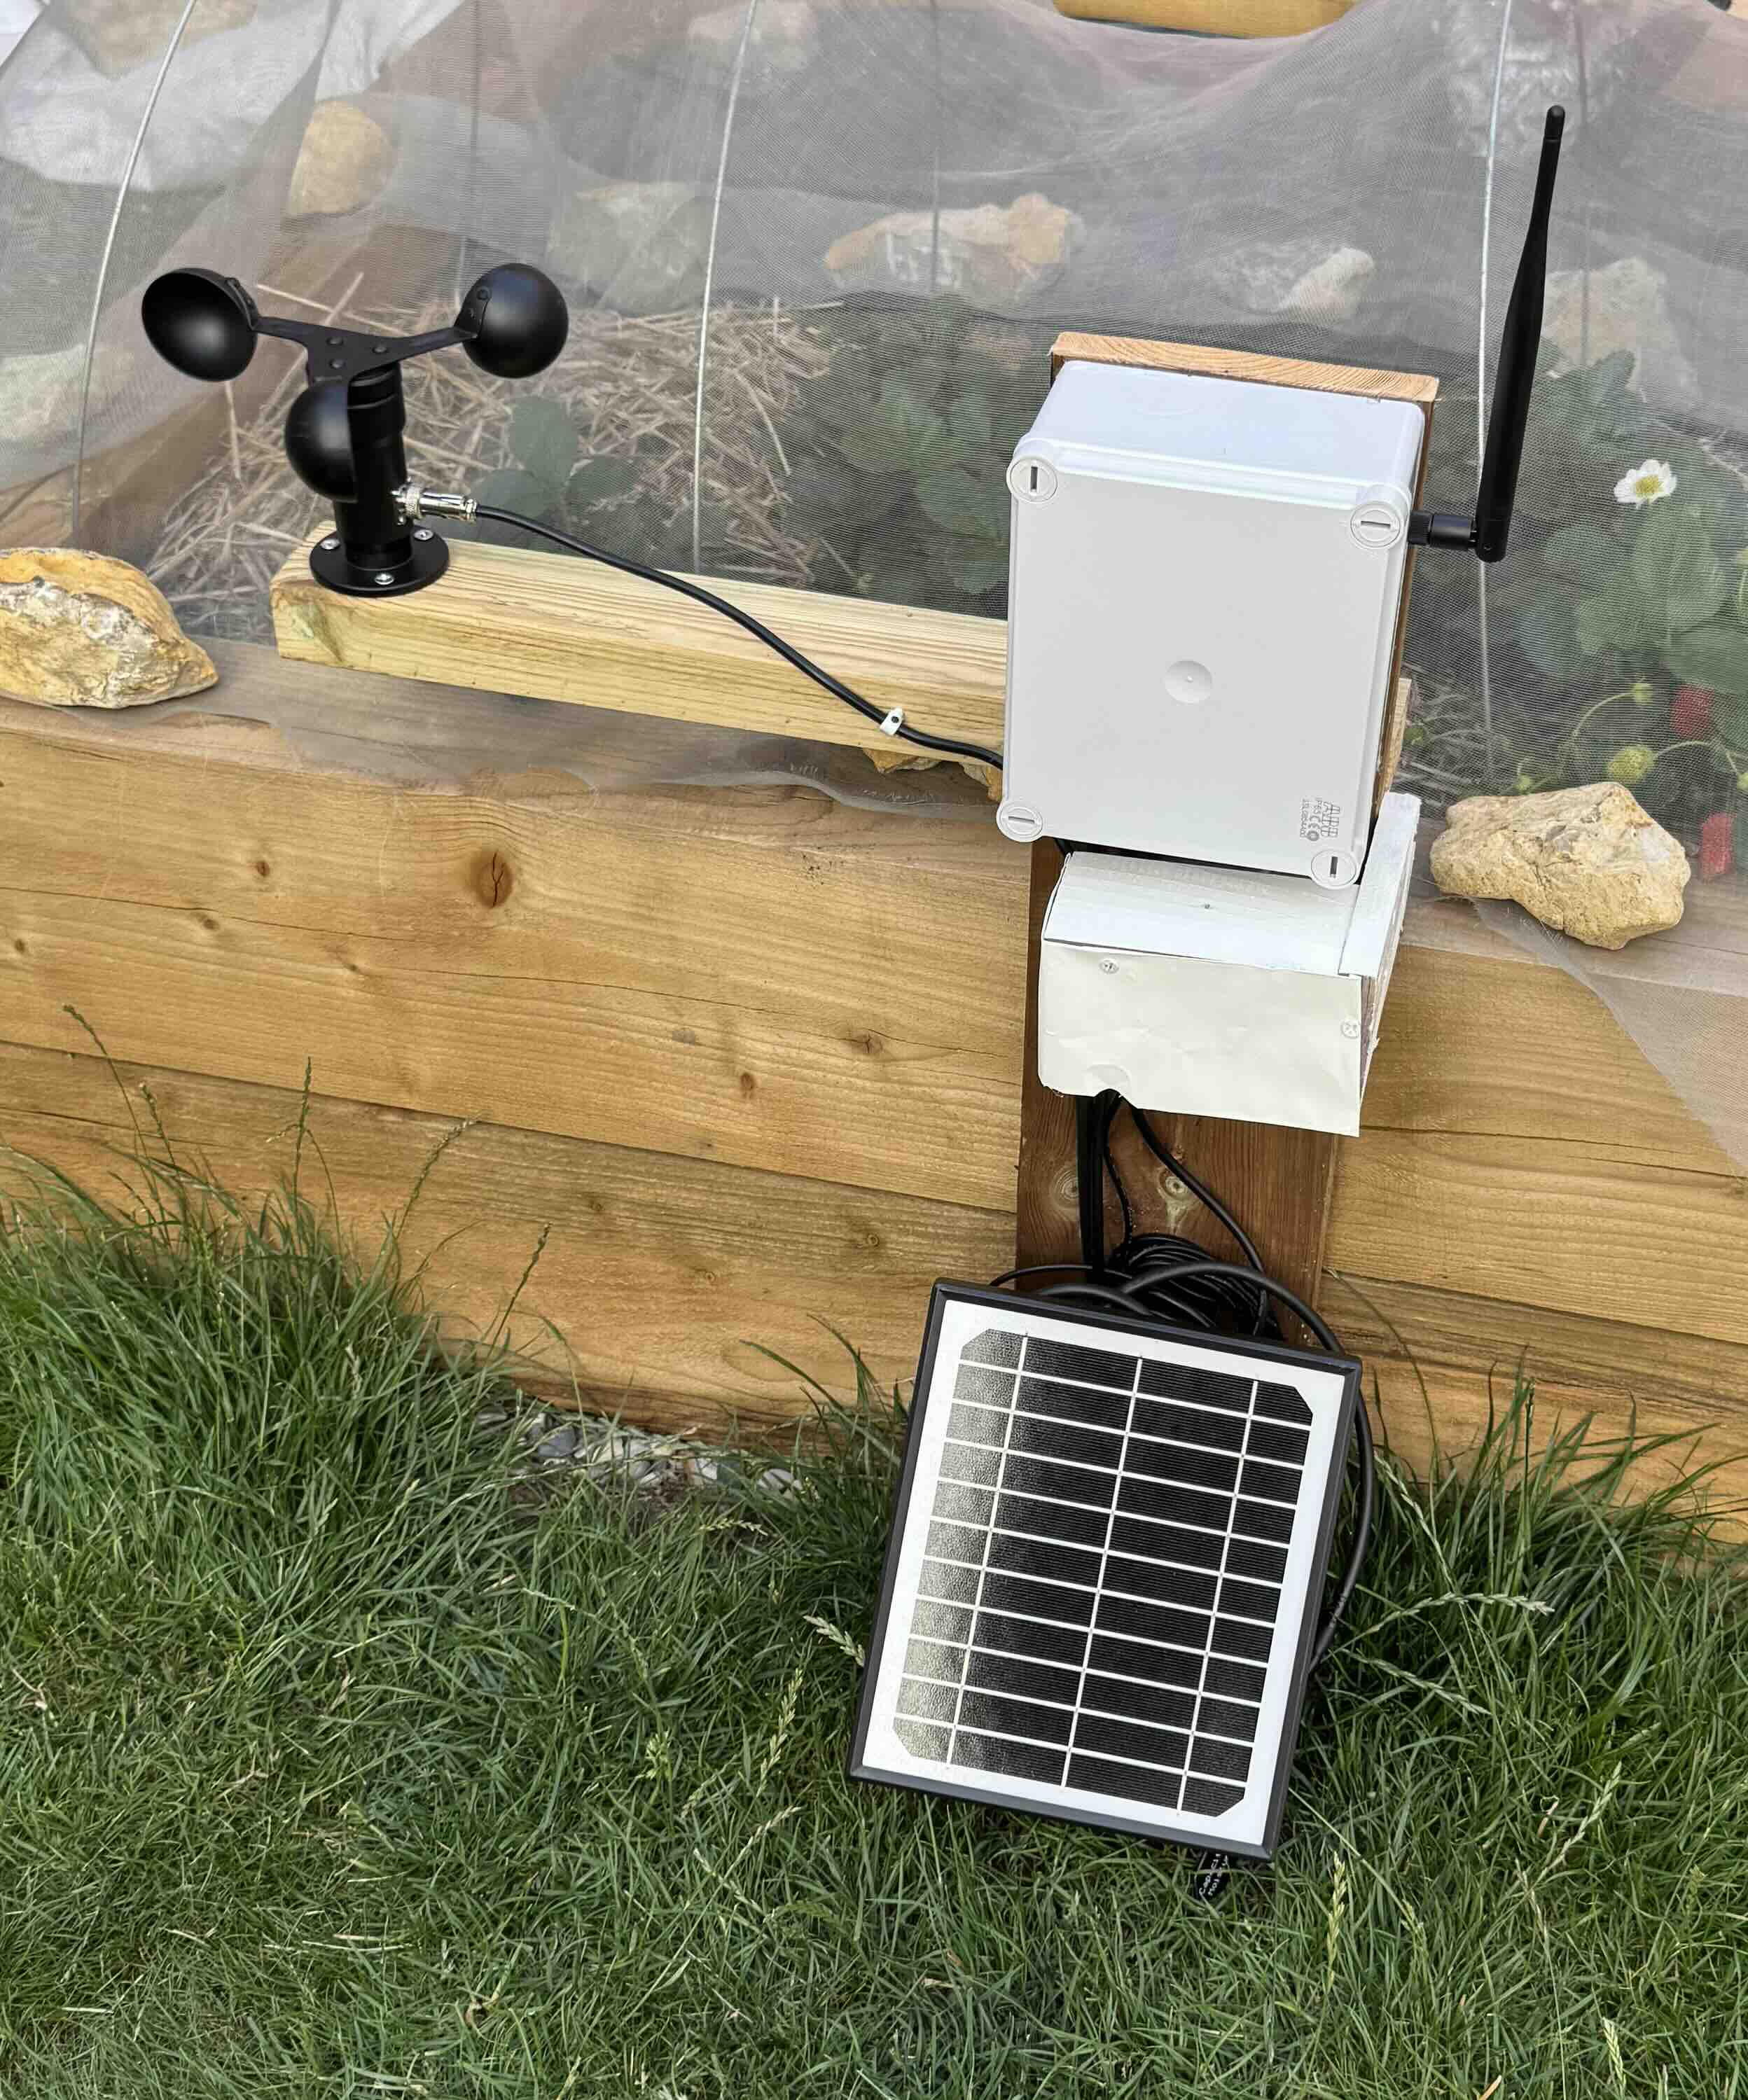
\includegraphics[width=0.5\textwidth]{figures/node.jpg}}
\caption{Sensor node}
\label{sensor-node}
\end{figure}

All components were commercially available, and assembling the final hardware
required only basic tools. Each device used the iLabs Challenger RP2040
microcontroller, which provided the necessary computing power and included
built-in LoRa capability for wireless communication. The gateway node was
additionally equipped with a Raspberry Pi to enable WIFI connectivity and remote
access via VNC Viewer.

\subsection{Webapp design}

Weather data was sent from the gateway to a purpose built webapp called
Agriscanner. This webapp allowed for the displaying of current, historic and
future (predicted) weather.

The dashboard (Figure \ref{dashboard}) displayed live weather data from the
nodes with a 1 minute update frequency. Clicking on a particular data point
allows the user to see a graph of past and future weather data in a way that is
familiar to any user of standard forecasting apps (Figure \ref{temperature}).

\begin{figure}[htbp]
\centerline{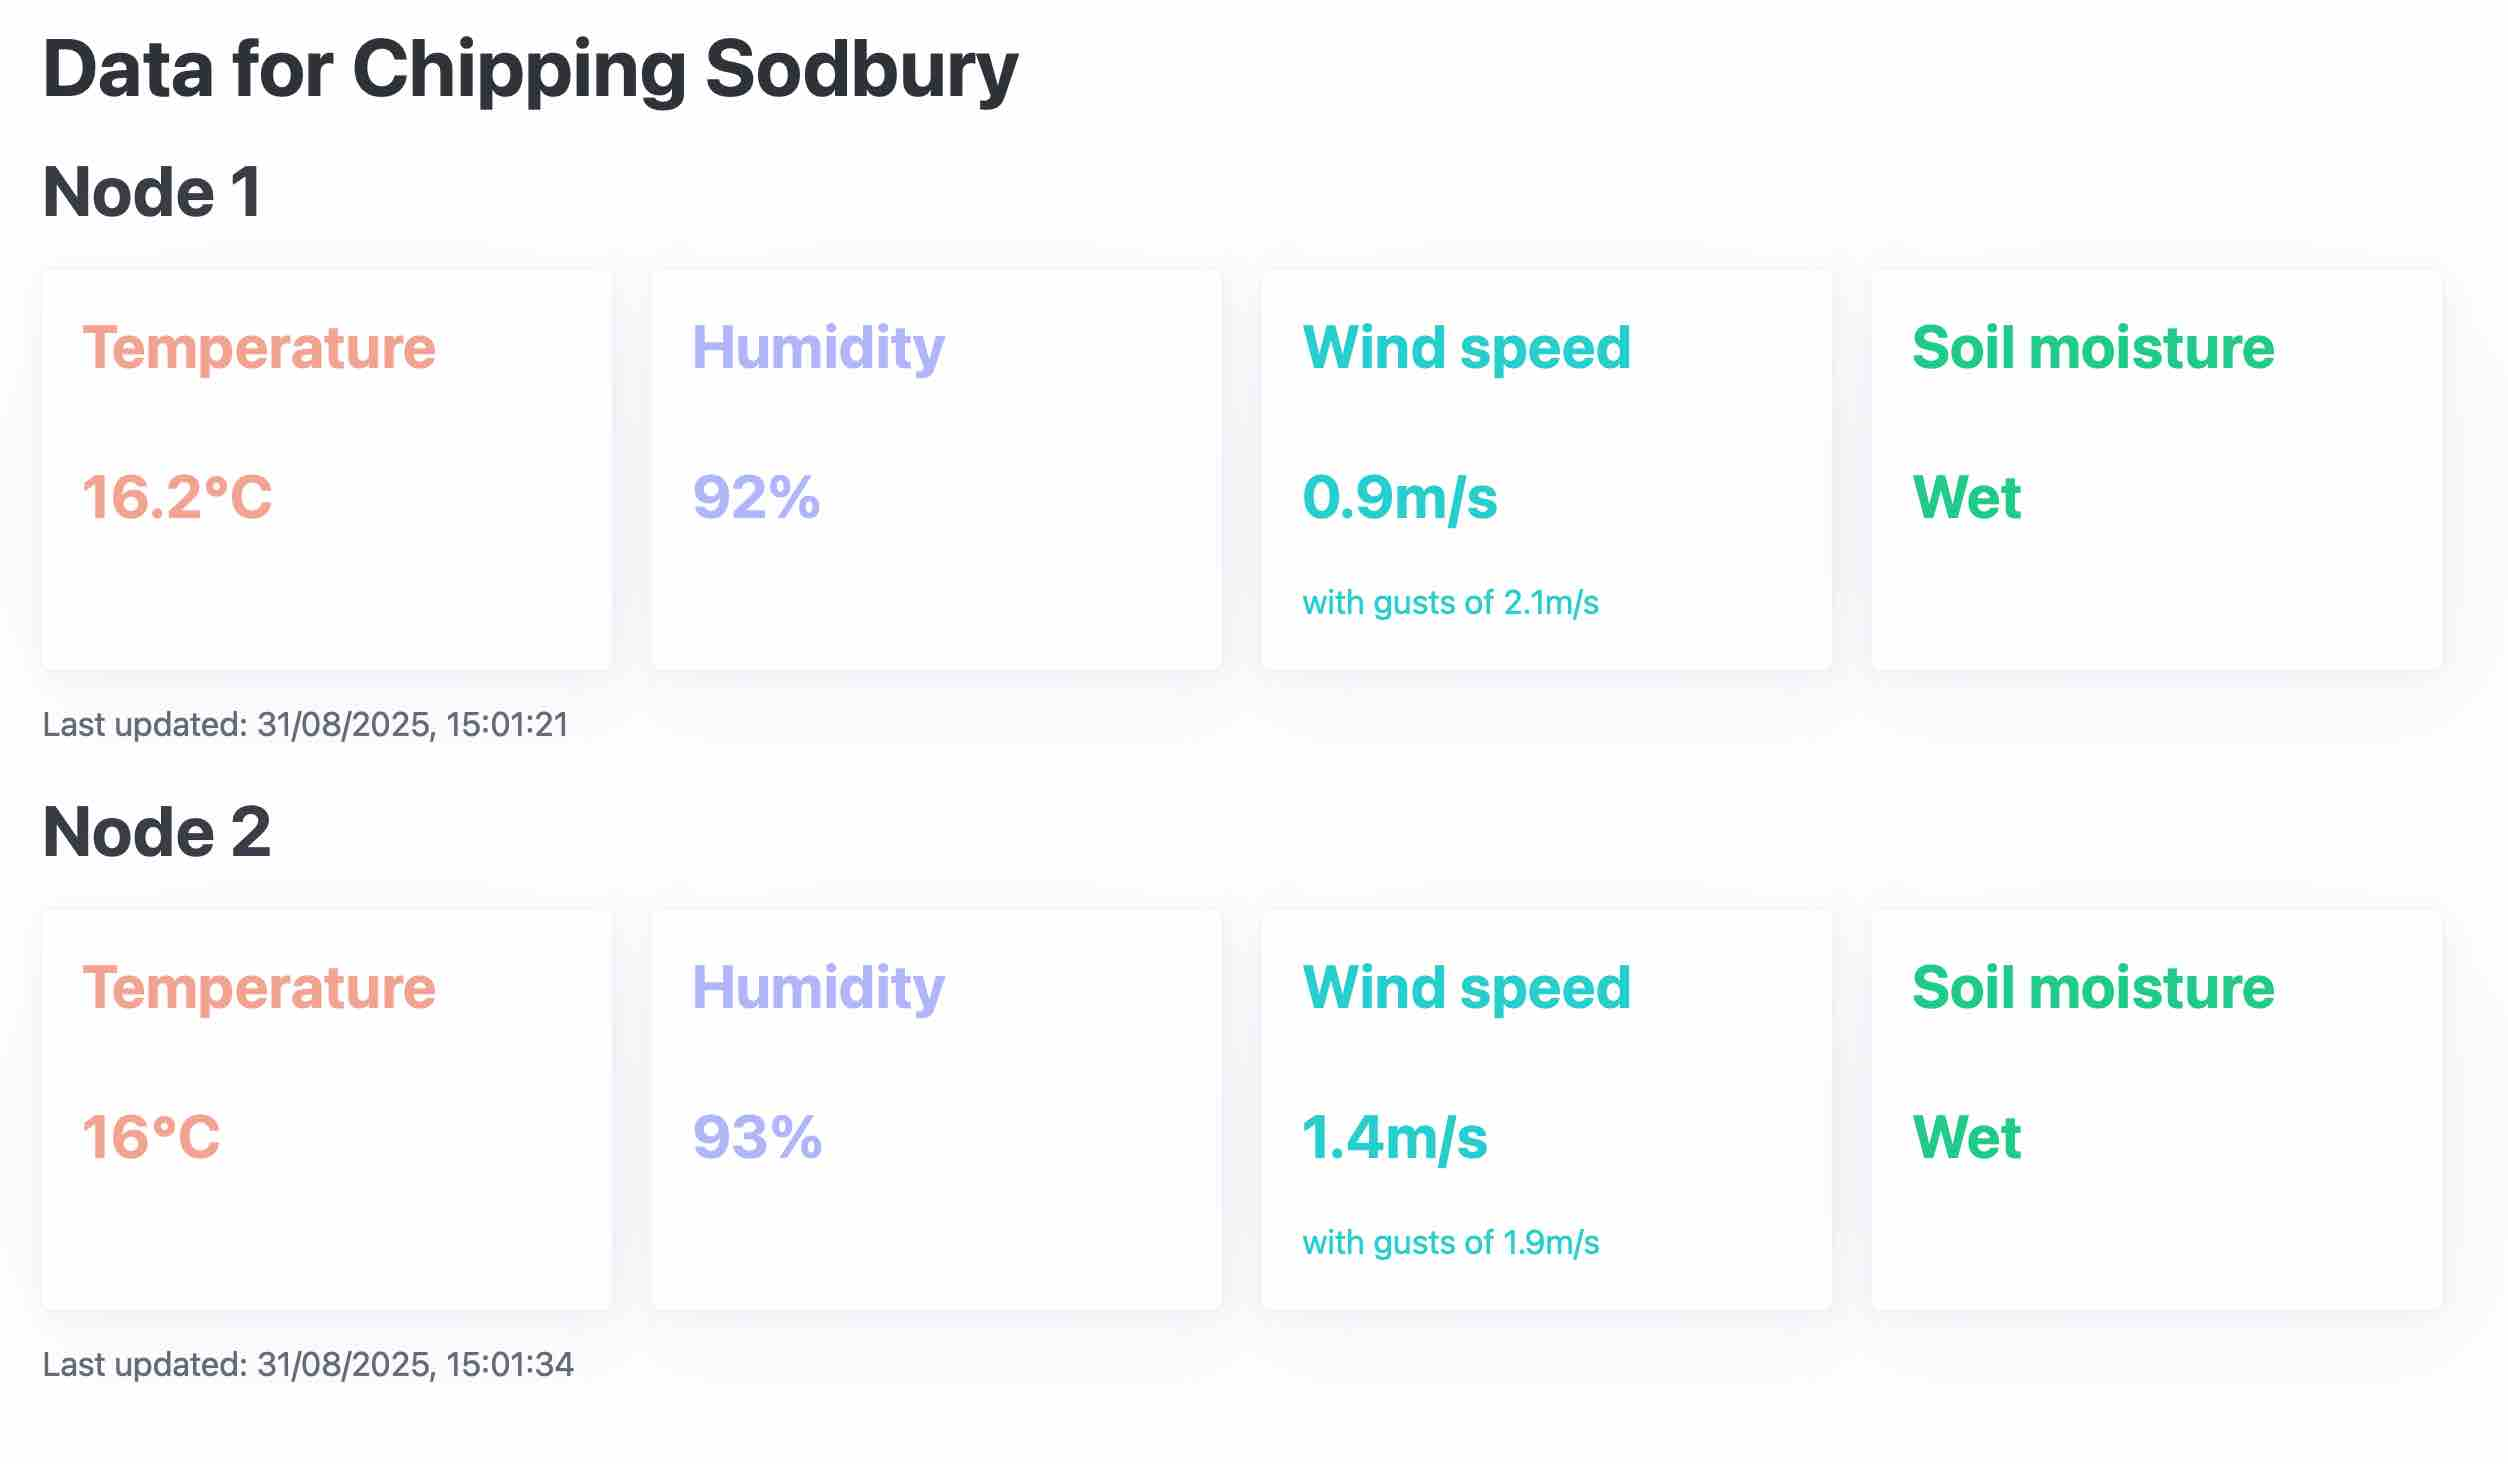
\includegraphics[width=0.5\textwidth]{figures/main-page.jpg}}
\caption{Webapp main dashboard}
\label{dashboard}
\end{figure}

\begin{figure}[htbp]
\centerline{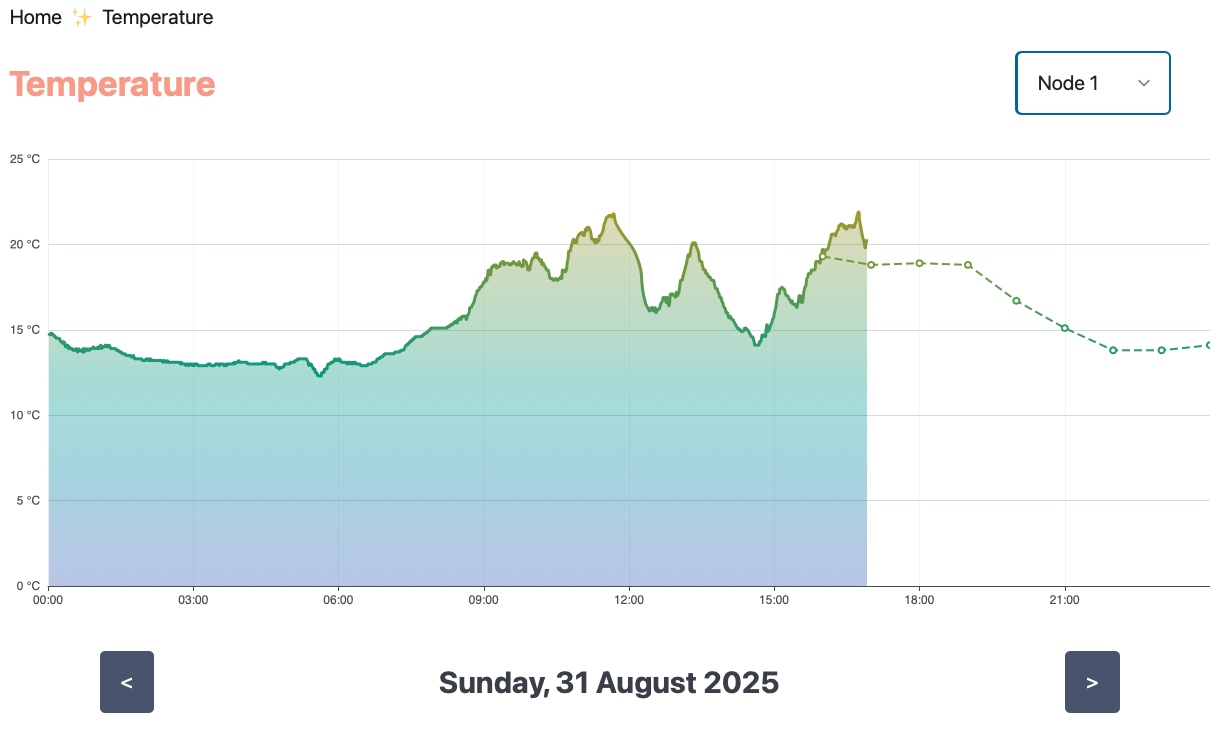
\includegraphics[width=0.5\textwidth]{figures/temperature-node-one.jpg}}
\caption{Webapp temperature page showing current and predicted weather}
\label{temperature}
\end{figure}

\subsection{Training and deployment of Machine learning algorithm}

To forecast microclimate date up to 48 hours in advance, we trained 10 separate
machine learning models using the LightGBM algorithm. One model was created for
each of the five sensor variables (temperature, humidity, wind speed, gust speed
and soil moisture) for each of the two nodes. LightGBM was selected for its high
performance on tabular climate data as the authors in
\cite{abdelmadjid2025enhancing} show. An additional benefit of this set up is
that LightGBM is compatible with the m2cgen library which allows the conversion
of the final models to individual JavaScript files.

\begin{figure}[htbp]
\centerline{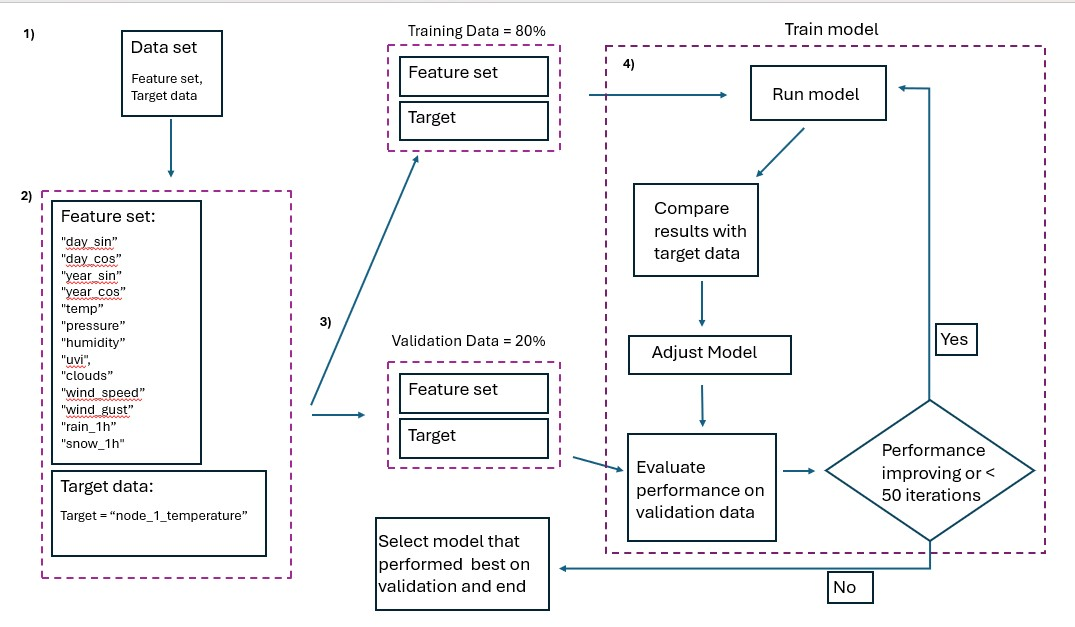
\includegraphics[width=0.5\textwidth]{figures/machine-learning-diagram2.jpg}}
\caption{Infographic showing training steps for training with LightGBM}
\label{machine-learning}
\end{figure}

The following steps were followed to train each of the ten models, this is also
shown visually in Figure \ref{machine-learning}

\begin{enumerate}
    \item \textbf{Dataset prepared:} A single cleaned dataset was created by
          matching timestamps between the api weather data and the sensor node
          data. As API readings are taken every 10 minutes and node readings
          every 1 minute, this meant that 9/10 node readings were discarded. The
          final dataset was roughly 1,400 rows. The data used for training
          spanned the period 15 - 27 August as that final date was when I
          trained the model.
    \item \textbf{Feature set and target data defined:} The feature set from the
          weather API and targets from the node data were defined, and
          unnecessary columns discarded. The database timestamp field was
          transformed into sine and cosine representations of day and year. This
          is necessary when training on a time-series data set as the algorithm
          must be able to understand the cyclical nature of time. For example,
          using raw timestamps would incorrectly suggest to the algorithm that
          the times of 23:00 on day 1 and 00:00 on day 2 are 23 hours apart
          rather than just 1 hour.
    \item \textbf{Dataset split into training data (80\%) and validation data
          (20\%):} The data is split by time so the training data consists of
          the first 80\% of the rows and the validation data the last 20\%. This
          data is then supplied to the model.
    \item \textbf{Iterative training:} For each iteration, the model looks at
          the inputs (training features) and the correct answers (training
          target) of the training rows, and determines where it is getting
          incorrect outputs. It builds a small decision tree that specifically
          aims to correct those mistakes on the training rows and adds that tree
          into itself so its predictions change a little. It then applies the
          updated model to the validation inputs (validation features) and
          compares those predictions to the validation answers (validation
          target) —to see how well the model would do on new "unseen" data. The
          validation data are never used to build the tree; they are only used
          to check the accuracy of the model. If the validation check shows no
          improvement after a number of iterations, the training stops and the
          model keeps the version that performed best on validation.  The
          process will perform a minimum of 50 iterations. I set the maximum
          number of iterations to 250 to prevent the models getting too large,
          as each iteration increases the model size substantially (The humidity
          model is over 40,000 lines long in JavaScript format for example).
\end{enumerate}

Once the ten models had been trained, they were uploaded to the web server. I
wrote an automated function on my backend that provides the models with
datapoints from the OpenWeather forecast data for the next 48 hours, and updates
this data every ten minutes to adjust the predictions as the forecast changes.
The outputs from the models are recorded as hourly predictions for each
datapoint in a JSON file, which is requested by the frontend software and used
to display a line graph of predicted values for the next 48 hours.

\section{Results}\label{RES}

\subsection{Machine learning performance}

\subsection{Range and cost}

\section{Conclusion}\label{CONC}

\subsection{Example figure and table}\label{FAT}

\begin{table}[htbp]
\caption{Table Type Styles}
\begin{center}
\begin{tabular}{|c|c|c|c|}
\hline
\textbf{Table}&\multicolumn{3}{|c|}{\textbf{Table Column Head}} \\
\cline{2-4} 
\textbf{Head} & \textbf{\textit{Table column subhead}}&
\textbf{\textit{Subhead}}& \textbf{\textit{Subhead}} \\
\hline
copy& More table copy$^{\mathrm{a}}$& &  \\
\hline
\multicolumn{4}{l}{$^{\mathrm{a}}$Sample of a Table footnote.}
\end{tabular}
\label{tab1}
\end{center}
\end{table}


\bibliography{references}

\end{document}
